\documentclass{article}
\usepackage[utf8]{inputenc}
\usepackage{mathtools}
\usepackage{amsfonts}
\usepackage{amssymb}
\usepackage{graphicx}
\usepackage{listings}
\usepackage{cite}

\title{An introduction to the Mandelbrot set}
\author{Bastian Fredriksson}
\date{January 2015}

\begin{document}

\maketitle

\section{Purpose and content}
The purpose of this paper is to introduce the reader to the very useful subject of fractals. We will focus on the Mandelbrot set and the related Julia sets. I will show some ways of visualising these sets and how to make a program that renders them. Finally, I will explain a key exchange algorithm based on what we have learnt.

\section{Introduction}
The Mandelbrot set and the Julia sets are sets of points in the complex plane. Julia sets were first studied by the French mathematicians Pierre Fatou and Gaston Julia in the early 20th century. However, at this point in time there were no computers, and this made it practically impossible to study the structure of the set more closely, since large amount of computational power was needed. 

Their discoveries was left in the dark until 1961, when a Jewish-Polish mathematician named Benoit Mandelbrot began his research at IBM. His task was to reduce the white noise that disturbed the transmission on telephony lines\cite{ibm}. It seemed like the noise came in bursts, sometimes there were a lot of disturbance, and sometimes there was no disturbance at all. Also, if you examined a period of time with a lot of noise-problems, you could still find periods without noise\cite{pritchard}. Could it be possible to come up with a model that explains when there is noise or not?

Mandelbrot took a quite radical approach to the problem at hand, and chose to visualise the data. The results showed a structure with self-similarity at all scales. This is called a fractal. There are many sorts of fractals, but what they all have in common are that they show signs of self-similarity. That means, when you zoom into the fractal, you will notice that some patterns repeat themselves. The fractal first studied by Mandelbrot was indeed the fractal generated by white noise from the telephony lines, also known as the Cantor dust fractal\cite{weisstein, ibm}.

All fractals can be generated using an Iterated Function System (IFS). An IFS consists of a function $f$ which is executed in a feedback loop, also known to computer students as a recursive function. That means, the output of the function is given as input when the function calls itself. The first time the function is called, you input some initial value $f(0)$\cite{fisher}. The Cantor dust fractal can be created using a black square as initial value. Each time you run the IFS in a feedback loop you split each square into four smaller squares and put them beside each other as shown in fig 1. 
\begin{figure}[ht!]
\centering
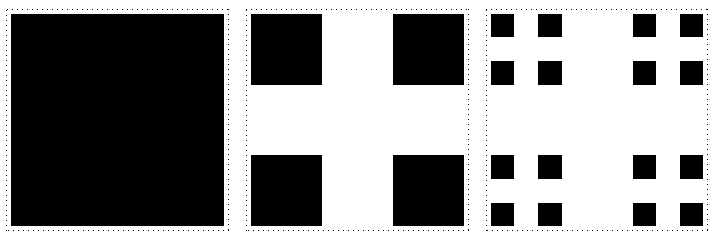
\includegraphics[width=120mm]{cantordust.png}
\caption{The Cantor dust fractal is generated by starting with a black square. In each iteration you split the square into four parts, thus creating clusters of "dust" which can be used to model white noise on telephony lines.\label{overflow}}
\end{figure}
If you repeat this process many times, you will eventually end up with a large amount of uniformly distributed dots, or "Cantor dust". The dots represents short periods of time where there is disturbance on the line. The dust appears, as you can see, in clusters. These clusters represents "a burst" of noise, periods of time where there is a lot of disturbance. The challenge for the engineers became to deal with these noise clusters and correct any errors as fast as possible\cite{pritchard}. The example with Cantor dust is just one example among many others, of phenomena in nature that can be modeled using fractals. Many other things, like a the helix of a shell or the surface of a broccoli prove to have fractal properties. There is even a theory called \textit{Fractal Cosmology} which states that the distribution of matter in the universe can be modeled as a fractal.
\section{The Mandelbrot set}
Encouraged by his findings, Benoit Mandelbrot continued his research at IBM. He began studying the work on Julia sets started by Pierre Fatou and Gaston Julia. With high-powered computers at his disposal he plotted the sets on paper. He noted that they were also fractals, with astonishing richness of detail. By making a small change to the IFS used by Fatou and Julia he came up with another fractal, which was later to be known as the Mandelbrot fractal or the Mandelbrot set. Benoit Mandelbrot wrote down his findings in the book \textit{The Fractal Geometry of Nature} which was published in 1982\cite{ibm}.

\subsection{Definition}
As I mentioned, the Mandelbrot set is a set of points in the complex plane. The complex plane is a two-dimensional space with the a vertical imaginary axis, and a horizontal real axis. A point in the plane can be described using a complex number $c\in \mathbb{C}$ written on the form $c=a+bi$ where $a,b\in \mathbb{R}$ and $i=\sqrt-1$. If you let the points belonging to the Mandelbrot set to be coloured in black, you obtain the shape depicted in figure 3.

Now we are ready to make a formal definition of the Mandelbrot set. A point $c \in \mathbb{C}$ belong to the Mandelbrot set iff
\[
\lim_{n\to \infty} || z_{n+1}=z_{n}^2+c || \nrightarrow \infty
\text{ where }z_{0}=0
\]

Here we have an IFS with the recursive formula $z_{n+1}=z_{n}+c$ and an initial value of $z_{0}=0$. In each loop, you square the previous number and seed the result with the value of $c$. The vertical brackets denotes the Euclidean norm, which is a measurement of how far away a point in the plane is from origo, $||z||=\sqrt{a^2+b^2}$. A point $c$ belongs to the Mandelbrot set if it remains bounded when we run the formula in a feedback loop. For example, the point $c=-1+0.25i$ belongs to the Mandelbrot set. If we apply the formula above, we retrieve the number series $z_{0}=0, z_{1}=-1+0.25i, z_{2}=-0.0625-0.25i, z_{3}\approx-0.059+0.281i, z_{4}\approx0.042-0.345i, z_{5}\approx-1.118+0.221i$ and so on. It is not obvious whether the point will eventually escape towards infinity or not, and it is usually not possible to tell. This is the reason why, in practical implementations, you run the feedback loop for a maximum number of times, say $n$ times. If the point still remains within a radius of 2 from origo you consider the point to belong to the set. Why 2? Well, it is possible to show, and this an important result, that if $||z_{n}||\ge 2$, $z_{n}$ will eventually escape towards infinity\cite{weisstein-mandelbrot}. This is called the \textit{bailout radius}. When you zoom into the set, you will notice that you will have to increase the size of $n$. This is why the rendering of fractals is such a time-consuming task.
\begin{figure}[ht]
\centering
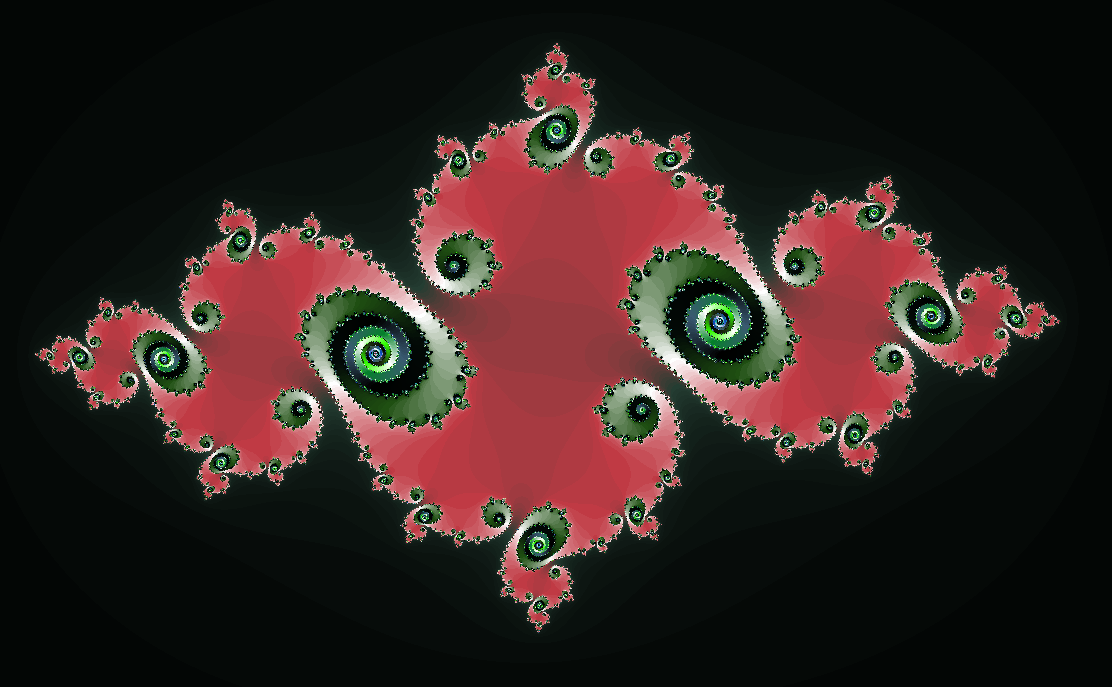
\includegraphics[width=120mm]{julia.png}
\caption{The Julia set generated from the seed $c=-0.755262+0.094211i$.}
\end{figure}
\subsection{Julia sets}
Julia sets and the Mandelbrot set are intrinsically connected through the fact that they are created using the same formula. This can be utilised to perform a cryptographic key exchange, see \textit{Application in cryptography}. While the Mandelbrot set is created using different values on $c$ and an initial value of $z_{0}=0$, a Julia set is created using a fixed $c$ as seed and different values on $z$. The complex number $c$ can be chosen freely\cite{alia&samsudin}.
If the point $c$ chosen does not belong to the Mandelbrot set, the resulting fractal will be a Cantor dust fractal. To determine whether a point $z$ belongs to the Julia set with seed $c$, iterate the formula $z_{n+1}=z_{n}+c$ in the same manner as with the Mandelbrot set.
\section{Exploring the set}
The Cantor dust fractal is not very exciting because it looks almost the same at all scales. The Mandelbrot fractal on the other hand is quite the opposite. When you zoom into the set, you will notice that new patterns emerge. The author has spent many hours zooming into the set, exploring new fascinating structures. 

The Mandelbrot set is actually a great example of how you can store an infinite amount of information on a finite medium. The prerequisite for creating an artistically appealing fractal lies in the existence of a colouring function $c(x)$. The purpose of the colouring function is often to colour the points which lies outside the set. This is called the aura of the Mandelbrot set. It is also possible to colour the set itself, although it is usually coloured in a fixed colour like black. In this section we will go through some methods of colouring and see what the result looks like.
\subsection{The escape time algorithm}
The most common algorithm for colouring the aura of the set is called the escape time algorithm. The escape time algorithm is based on the value of $n$, that means, the number of iterations before $z_{n}$ end up outside the bailout radius. A simple, yet beautiful way of colouring, is to colour the actual set in black and then fade the aura from red to black. One way of defining the colouring function would then be:
\[
c(n) = \begin{cases}
0 & n = max(n) \\
255 - n / max(n) + 1 & n < max(n)
\end{cases}
\]

$c(n)$ returns the red component of a RGB-colour. If you want be able to colour your fractal in many different colours, it is often convenient to use three functions, $c_{r}(x)$, $c_{g}(x)$ and $c_{b}(x)$ where $c_{r}$ returns the red component, $c_{g}$ returns the green component and $c_{b}$ returns the blue component. Another approach is to prepare a colour palette, and then let the function $c(x)$ point out a colour in the palette. In this way, you can create e.g. rainbow effects.

\begin{figure}
\centering
\begin{minipage}[ht]{.45\textwidth}
\centering
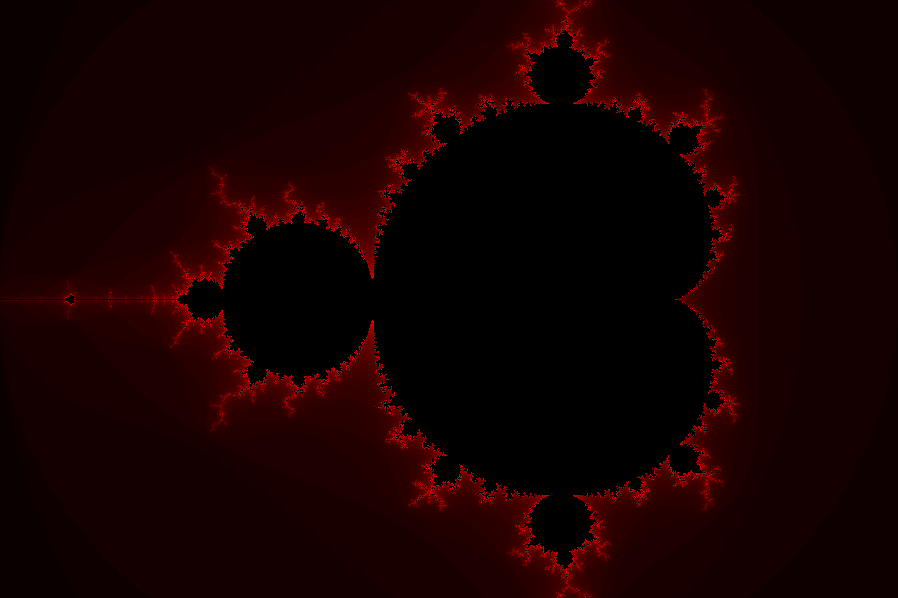
\includegraphics[width=1.0\textwidth,height=3.5cm]{mandelbrot.png}
\caption{The aura of the set coloured using the traditional escape time algorithm. The black bulb in the middle is the actual Mandelbrot set.}
\end{minipage}\hfill
\begin{minipage}[ht]{.45\textwidth}
\centering
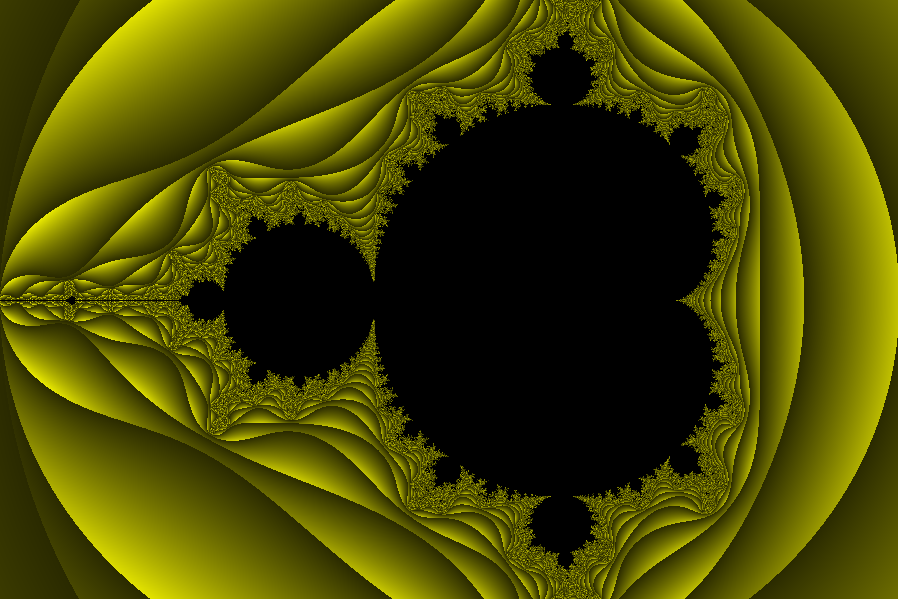
\includegraphics[width=1.0\textwidth,height=3.5cm]{abs.png}
\caption{The aura coloured by measuring the distance from origo and scaling it with a constant.\\\\}
\end{minipage}
\end{figure}

\begin{figure}
\centering
\begin{minipage}[ht]{.45\textwidth}
\centering
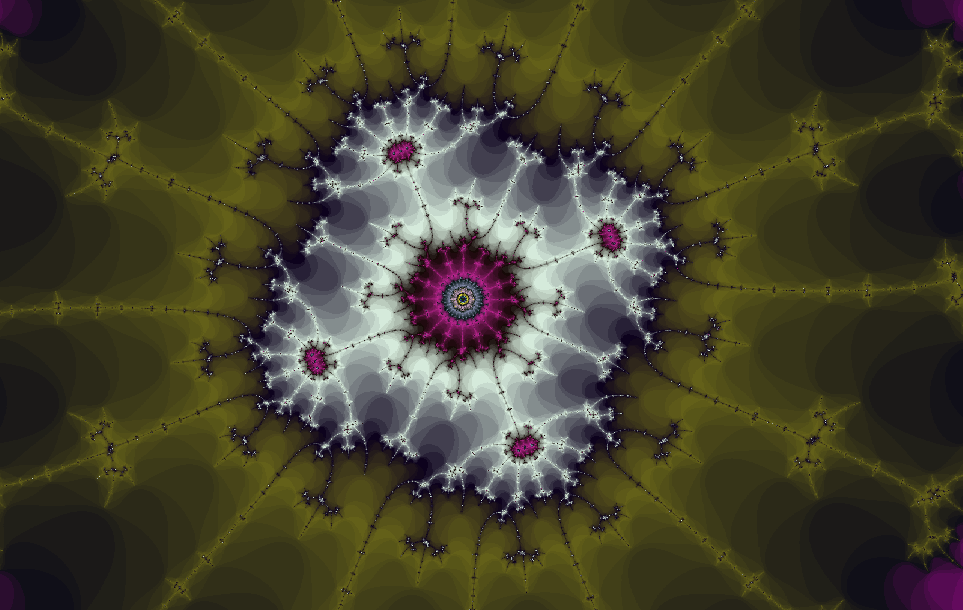
\includegraphics[width=1.0\textwidth,height=3.5cm]{palette.png}
\caption{Part of the Mandelbrot set coloured with a palette.}
\end{minipage}\hfill
\begin{minipage}[ht]{.45\textwidth}
\centering
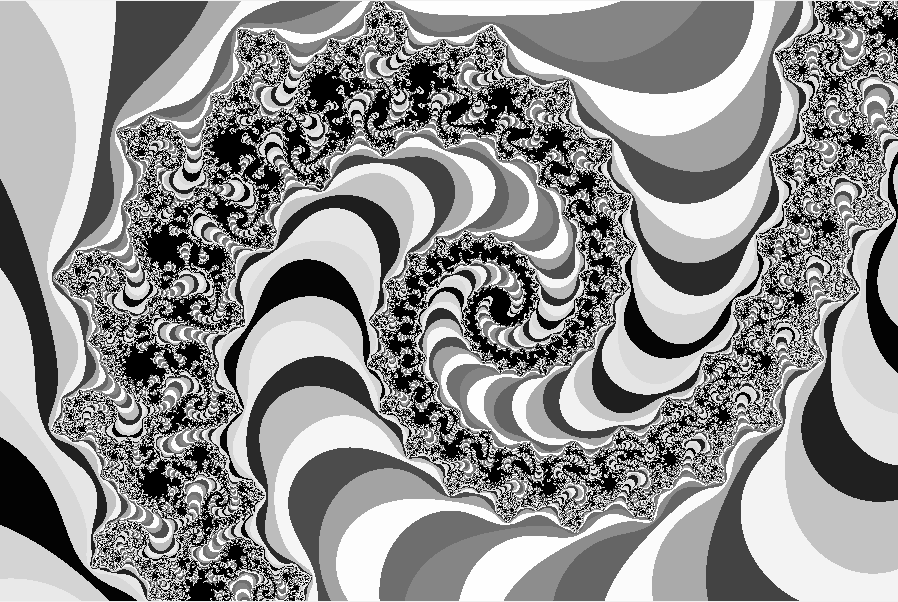
\includegraphics[width=1.0\textwidth,height=3.5cm]{cosine.png}
\caption{A Mandelbrot spiral coloured using cosine.}
\end{minipage}
\end{figure}

\begin{figure}[ht]
\centering
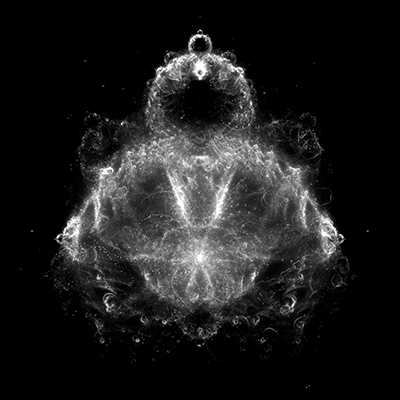
\includegraphics[width=120mm]{buddhabrot.png}
\caption{A Buddhabrot generated with $n=10^6$\cite{unreifekirsche}}.
\end{figure}

\subsection{Buddhabrot}
Another variant of the Mandelbrot set is the Buddhabrot. The name arises from the fact that the fractal looks like a meditating Buddha. An image of a Buddhabrot was first posted by Melinda Green on Usenet in 1993\cite{wikipedia}. At first glance it does not look like a Mandelbrot at all, but it is only the colouring that differs. Instead of counting the number of iterations required, like in the escape time algorithm, you count the number of times a specific point has been visited. The fractal is rendered by splitting the canvas into a matrix $M$, where each element in the matrix represents the number of times this area of the fractal has been visited. For each output from the function $z_{n}$ you increment the number on the corresponding position in the matrix. Once you have executed $z_{n}$ for all possible $c$ you make a second pass over M. Here you can use a colouring function $c(x)$ similar to what we described in section 3.1 to map the elements in M to colours.
\section{Implementation}
This section contains sample code written in C\# to get you started rendering your own fractals.
Begin by creating a canvas with a size of $n\times m$ pixels. Each pixel represents a unique $c$. Transform the position of the pixel on screen to a complex number in the plane. Given that the coordinates of the complex number can be written as $(x, y)$ and the plane has the following boundaries; $x_{min}\le x \le x_{max}$ and $y_{min} \le y \le y_{max}$, the transformation functions could look something like this:
\begin{lstlisting}[language=C]
double trans_x(double x, double x_min, double x_max) {
    return x / (m / (x_max - x_min)) + x_min;
}

double trans_y(double y, double x_min, double x_max) {
    return y_max - y / (n / (y_max - y_min));
}
\end{lstlisting}
Now, for each pixel in your canvas, iterate the formula $z_{n+1}=z_{n}+c$ until $z_{n}$ falls outside the bailout radius or until $n=max(n)$. Depending on how you want to colour your fractal you might either store the counter $n$ or some other information you need to remember. In the example below, a complex number is represented using two doubles, where $re$ is the real part and $im$ is the coefficient for the imaginary part.
\begin{lstlisting}[language=C]
for (int y = 0; y < n; y++) {
    for (int x = 0; x < m; x++) {
        double re = 0; // z_{n+1} 
        double im = 0;
        double re_old = 0; // z_{n}
        double im_old = 0;
        double a = trans_x(x, x_min, x_max);
        double b = trans_y(y, y_min, y_max);
        int n;
        for (n = 0; Math.Pow(re, 2) + 
            Math.Pow(im, 2) < 4 && n < N_MAX; n++) {
            // z_{n+1}=z_{n}^2+c
            re_old = Math.Pow(re, 2) - Math.Pow(im, 2);
            im_old = 2.0 * re * im;
            re = a + re_old;
            im = b + im_old;
        }
        colour_pixel(x, y, n);
    }
}
\end{lstlisting}
\subsection{Optimisations}
You might have noticed that we have done the transformation \[||z||=\sqrt{x^2+y^2} \to ||z||^2=x^2+y^2\] to avoid the time consuming square root function. Other optimisations you can do is to split the canvas into say, blocks of $n/10\times m/10$ pixels, and calculate each block in its own thread. This should speed up calculations a lot, since you exploit all cores in the CPU. You can also use a technique called periodicity checking. Each number series given by calculating $z_{n}$ for different $n$ can be seen as an orbit. If there is a cycle in the orbit, then we know that $z_{n}$ cannot diverge when $n \to \infty$, hence the point must be a part of the Mandelbrot set. However, cycle checking with floating point arithmetic is difficult and if you do not get it right, you might end up with a program running even slower, so I would not recommend this kind of optimisation unless you really need speed\cite{xaos}. You can also decrease the bailout radius, but be careful, the results can be inaccurate. Another thing you could try is to do the calculations on your graphics card. Fractals should be suitable for graphic cards, since they are better at floating point arithmetic's, and since it is easy to split computations into smaller pieces.
\begin{figure}[hb]
\centering
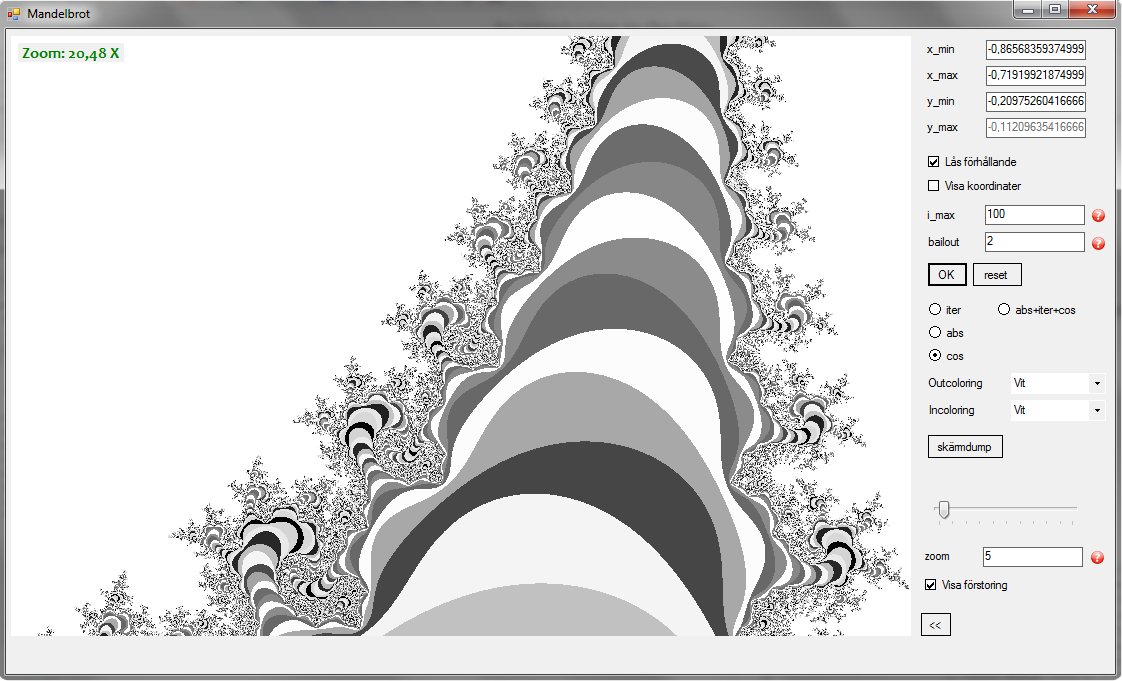
\includegraphics[width=120mm]{program.png}
\caption{The Windows program \textit{Mandelbrot} made by the author. If you do not want to make your own program, you can try \textit{XaoS} or \textit{Fractal eXtreme}.}
\end{figure}
\section{Application in cryptography}
Fractals is not only about beautiful images and computer graphics. The chaotic nature of fractals have made them suitable for cryptographic applications such as hash functions and encryption. In this section, we will go through a key exchange protocol based on the Mandelbrot set.
\subsection{Fractal key exchange}
In cryptography, a key exchange is the process of two parties, Alice and Bob, exchanging keys with each other allowing the use of a cryptographic algorithm. This is done through a key exchange protocol such as Diffie-Hellman. Diffie-Hellman has an important property; even if Eve is eavesdropping on the traffic sent between Alice and Bob, she cannot deduct the common secret. This is what makes Diffie-Hellman secure. Computer security researchers Mohammad Ahmad Alia and Azman Bin Samsudin at University Sains Malaysia have invented a new type of key exchange protocol which utilises floating point arithmetics\cite{alia&samsudin}. The protocol is very similar to Diffie-Hellman, and relies on the following equivalence relation:
\[
c^{n-x}q_{n}e=c^{k-x}q_{k}d\quad \forall x\in \mathbb{Z} 
\text{ where } c, d, e\in \mathbb{C} \text{ and }
n, k\in \mathbb{N}
\]
Where $q_{i}\in \mathbb{C}$ is the result from running  $q$ in a feedback loop $i$ times. $p_{a}$ and $p_{b}$ as defined below are the public keys for Alice and Bob respectively.
\begin{enumerate}
  \item The proposed protocol begins with Alice and Bob agreeing on a complex number $c$ which belongs to the Mandelbrot set and an integer $x$. $c$ and $x$ are public and can be intercepted by a third party without compromising the protocol.
  \item Alice generates her secret key consisting of the tuple $(n, e)$ where $n>x$ and $e$ belongs to the Mandelbrot set.
  \item Bob generates his set key consisting of the tuple $(k, d)$ where $k>x$ and $d$ belongs to the Mandelbrot set.
  \item Alice calculates $z_{n}$ by iterating the formula $z_{i+1}=z_{i}c^2e$, $z_{0}=c$ (1) $n$ times and sends $p_{a}=z_{n}e$ to Bob.
  \item Bob calculates $z_{k}$ by iterating the formula $z_{i+1}=z_{i}c^2d$, $z_{0}=c$ (1) $k$ times and sends $p_{b}=z_{k}d$ to Alice.
  \item Alice calculates the common secret $c^{n-x}q_{n}e$ by iterating the formula $q_{i+1}=q_{i}ce$, $q_{0}=p_{b}$ (2) n times.
  \item Bob calculates the common secret $c^{k-x}q_{k}d$ by iterating the formula $q_{i+1}=q_{i}cd$, $q_{0}=p_{a}$ (2) k times.
\end{enumerate}
The function (1) is called \textit{Mandelfn} and the function (2) is called \textit{Juliafn} because they bore a slight resemblance to the original Mandelbrot and Julia functions.

The keyspace, given a key with length $n$, is larger for the fractal key exchange algorithm than the keyspace for Diffie-Hellman, because the keyspace of Diffie-Hellman is limited to the number of primes in the field $\mathbb{Z}_{p}$ where $p$ is the largest prime that can be represented by $2^n$ bits. However, using the fractal key exchange algorithm we can potentially end up with any key, which means that the keyspace is exactly $2^n$. The fractal approach also has an interesting property. The values of $n$ and $k$ can be seen as a \textit{load factor} that will slow down the calculations and increase the security of the protocol.
\begin{figure}[hb]
\centering
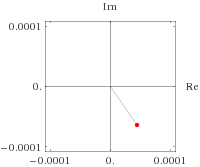
\includegraphics[width=50mm]{key.png}
\caption{The common secret plotted in the complex plane.}
\end{figure}

\subsection{An example}
\begin{enumerate}
\item We choose $c=-0.6+0.12i$ and $x=1$.
\item We let Alice's private key consist of $n=2$ and $e=-0.1+0.72i$.
\item We let Bob's private key consist of $k=3$ and $d=0.21-0.35i$.
\item $z_{1}=c^3e$\\
$z_{2}=c^5e^2$\\
We send $p_{a}=c^5e^3$ to Bob.
\item $z_{1}=c^3d$\\
$z_{2}=c^5d^2$\\
$z_{3}=c^7d^3$\\
We send $p_{b}=c^7d^4$ to Alice.
\item $q_{1}=c^8d^4e$ \\
$q_{2}=c^9d^4e^2$\\
The common secret becomes:\\ $cq_{3}e=c^{10}d^4e^3\approx 0.0000443966-0.0000646526i$.
\item $q_{1}=c^6e^3d$\\
$q_{2}=c^7e^3d^2$\\
$q_{3}=c^8e^3d^3$\\
The common secret becomes:\\ $c^2q_{3}d=c^{10}e^3d^4\approx 0.0000443966-0.0000646526i$.
\end{enumerate}

\section{Conclusion}
I hope the reader has gained some insight about the Mandelbrot set. As shown in the paper, it has several practical applications, not only in computer graphics. The fractal is like pi, it shows up even when you least expect it to. This paper is, as the title suggests, only an introduction to the Mandelbrot set and fractals in general. There are many other cool things you can do with fractals. One example of a recent discovery in the field of fractals was made by Tom Lowe in 2010 when he discovered the 3-dimensional Mandelbox. Although it has never reached any commercial success, studies has shown that fractals are suitable for image compression. If you are interested in the subject, you might take a look in \textit{References}. You can also try to enhance the key exchange algorithm described in section 5.

\newpage
\bibliographystyle{acm}
\bibliography{refs}

\begin{figure}[ht!]

\includegraphics[width=40mm]{bastian.jpg}
\end{figure}
\noindent
Bastian Fredriksson began his studies at The Royal University of Technology in 2012. He is currently studying his third year on the Bachelor's Programme in Computer Science.
\end{document}